\documentclass[12pt]{article}

\include{preamble}

\newtoggle{solutions}
%\toggletrue{solutions}

\title{Math 343 / 643 Fall \the\year{} \\ Midterm Examination One}
\author{Professor Adam Kapelner}
\date{March 4, \the\year{}}

\begin{document}
\maketitle

\noindent Full Name \line(1,0){410}

\thispagestyle{empty}

\section*{Code of Academic Integrity}

\footnotesize
Since the college is an academic community, its fundamental purpose is the pursuit of knowledge. Essential to the success of this educational mission is a commitment to the principles of academic integrity. Every member of the college community is responsible for upholding the highest standards of honesty at all times. Students, as members of the community, are also responsible for adhering to the principles and spirit of the following Code of Academic Integrity.

Activities that have the effect or intention of interfering with education, pursuit of knowledge, or fair evaluation of a student's performance are prohibited. Examples of such activities include but are not limited to the following definitions:

\paragraph{Cheating} Using or attempting to use unauthorized assistance, material, or study aids in examinations or other academic work or preventing, or attempting to prevent, another from using authorized assistance, material, or study aids. Example: using an unauthorized cheat sheet in a quiz or exam, altering a graded exam and resubmitting it for a better grade, etc.\\
\\
\noindent I acknowledge and agree to uphold this Code of Academic Integrity. \\~\\

\begin{center}
\line(1,0){350} ~~~ \line(1,0){100}\\
~~~~~~~~~~~~~~~~~~~~~~~~~~~~~~~~~~signature~~~~~~~~~~~~~~~~~~~~~~~~~~~~~~~~~~~~~~~~~~~~~~~~~~~~~~~~~~~~~~ date
\end{center}

\normalsize

\section*{Instructions}
This exam is 75 minutes (variable time per question) and closed-book. You are allowed \textbf{one} page (front and back) of a \qu{cheat sheet}, blank scrap paper (provided by the proctor) and a graphing calculator (which is not your smartphone). Please read the questions carefully. Within each problem, I recommend considering the questions that are easy first and then circling back to evaluate the harder ones. No food is allowed, only drinks. %If the question reads \qu{compute,} this means the solution will be a number otherwise you can leave the answer in \textit{any} widely accepted mathematical notation which could be resolved to an exact or approximate number with the use of a computer. I advise you to skip problems marked \qu{[Extra Credit]} until you have finished the other questions on the exam, then loop back and plug in all the holes. I also advise you to use pencil. The exam is 100 points total plus extra credit. Partial credit will be granted for incomplete answers on most of the questions. \fbox{Box} in your final answers. Good luck!

\pagebreak

\problem We are modeling the number of successful sales out of a known $m$ daily cold calls made by a sales team. We observe the number of sales over $n$ days, denoted by $\x := \braces{\xoneton}$, where each $x_i \in \braces{0, 1, \dots, m}$. 

We suspect a \qu{hurdle} effect: some days are complete busts due to market conditions (0 sales), but if the team gets past that hurdle and makes at least one sale, the total number of sales follows a Binomial distribution. We use a \textit{Binomial Hurdle} model. With probability $\theta_1$, a day yields strictly 0 sales. With probability $1 - \theta_1$, the day yields $x_i > 0$ sales, drawn from a Zero-Truncated Binomial (ZTBin) distribution, 

\beqn
X \sim \text{ZTBin}(m, \theta) := \frac{\displaystyle\binom{m}{x} \theta^{x} (1-\theta)^{m-x}}{1 - (1-\theta)^m} \indic{x \in \braces{1, 2, \ldots, m}},~~ \expe{X} = \frac{m\theta}{1 - (1-\theta)^m}
\eeqn

\noindent Thus, the DGP for the observed $\Xoneton$ is iid:

\beqn
\prob{X = 0} &=& \theta_1 \\
\prob{X = y} &=& \parens{1 - \theta_1}\text{ZTBin}(m, \theta_2)
\eeqn

\noindent Let $n_0 :=$ be the number of days with exactly 0 sales, and $n_+ :=$ be the number of days with strictly $>0$ sales (such that $n_0 + n_+ = n$). Also let $s := \sum_{\braces{i: x_i > 0}} x_i$.

\begin{enumerate}[(a)]

\subquestionwithpoints{2} What are the parameter(s) in this model?

\iftoggle{solutions}{\inred{
$\theta_1, \theta_2$
}}{~\spc{0}}

\subquestionwithpoints{6} Write the likelihood function $f$ for all $n$ observations.
%
\iftoggle{solutions}{\inred{
\beqn
f(\x~|~\theta_1, \theta_2) &=& \prod_{\braces{i: x_i = 0}} \theta_1 \prod_{\braces{i: x_i > 0}} (1 - \theta_1) \frac{\binom{m}{x_i} \theta_2^{x_i} (1-\theta_2)^{m-x_i}}{1 - (1-\theta_2)^m}  \\
&=& \theta_1^{n_0} \tothepow{\frac{1 - \theta_1}{1 - (1-\theta_2)^m}}{n_+} \parens{\prod_{\braces{i: x_i > 0}} \binom{m}{x_i}} \tothepow{\frac{\theta_2}{1-\theta_2}}{s} \tothepow{1 - \theta_2}{mn_+}
\eeqn
}}{~\spc{10}}
\pagebreak


\subquestionwithpoints{3} Assume Laplace priors for the parameter(s). Write those priors below. If they are improper, then write them as proportionalities below.

\iftoggle{solutions}{\inred{
\beqn
\theta_1 \sim \stduniform,~~ \theta_2  \sim \stduniform
\eeqn
}}{~\spc{0}}

\subquestionwithpoints{5} Derive the kernel of the conditional posterior distribution of $\theta_1$ given $\theta_2$ and the data. Use the priors from (c). Don't forget the indicator function for $\theta_1$.

\iftoggle{solutions}{\inred{
\beqn
f(\theta_1 ~|~ \theta_2, \x) \propto \theta_1^{n_0} \tothepow{1 - \theta_1}{n_+} \indic{\theta_1 \in (0,1)}
\eeqn
}}{~\spc{3}}

\subquestionwithpoints{2} Is the kernel in the previous question correspond to a known distribution? If so, provide that distribution below. If not, write \qu{no} below.

\iftoggle{solutions}{\inred{
\beqn
f(\theta_1 ~|~ \theta_2, \x) = \betanot{n_0 + 1}{n_+ + 1}
\eeqn
}}{~\spc{1}}


\subquestionwithpoints{6} Derive the kernel of the conditional posterior distribution of $\theta_2$ given $\theta_1$ and the data. Use the priors from (c).  Don't forget the indicator function for $\theta_2$.

\iftoggle{solutions}{\inred{
\beqn
f(\theta_2 ~|~ \theta_1, \x) &\propto& \tothepow{\frac{1}{1 - (1-\theta_2)^m}}{n_+} \tothepow{\frac{\theta_2}{1-\theta_2}}{s} \tothepow{1 - \theta_2}{mn_+}  \indic{\theta_2 \in (0,1)} \\
&=& \tothepow{1 - (1-\theta_2)^m}{-n_+} \theta_2^s \tothepow{1-\theta_2}{mn_+ - s}   \indic{\theta_2 \in (0,1)}
\eeqn
}}{~\spc{6.5}}


\subquestionwithpoints{2} Is the kernel in the previous question correspond to a known distribution? If so, provide that distribution below. If not, write \qu{no} below.

\iftoggle{solutions}{\inred{
No
}}{~\spc{1}}
\pagebreak

\subquestionwithpoints{3} As of now, can we use a Gibbs Sampler to draw samples from the posterior distribution? Yes/no and why?

\iftoggle{solutions}{\inred{
No, because we need to be able to sample from all conditional distributions. We can only sample from the first.
}}{~\spc{1}}


Regardless of what you wrote for answers in (e) and (g), we implement a sampler for the posterior distribution and we sample 2,000 draws.  In our example, $m=15$.

\subquestionwithpoints{3} Below is a scatterplot where the $x$ denotes sampling iteration number the $y$ axis displays samples of $\theta_1$ given $\x$.

\begin{figure}[h]
    \centering
    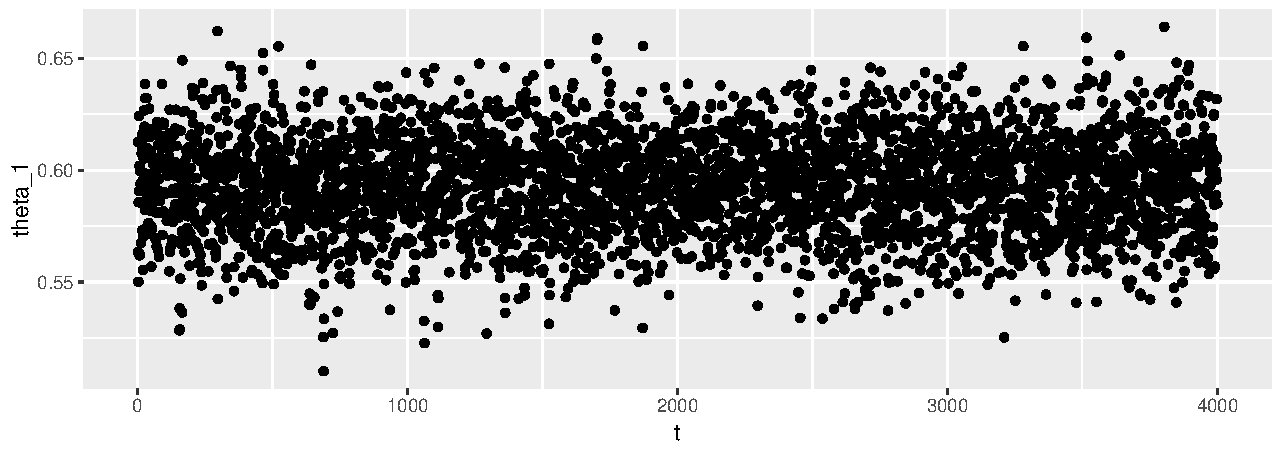
\includegraphics[width=1\linewidth]{theta_1_burn.pdf}
\end{figure}

Do we need to burn a certain number of initial samples? If yes, write the approximate iteration number. If no, write zero.

\iftoggle{solutions}{\inred{
0
}}{~\spc{1}}
\pagebreak


Below is an autocorrelation plot for the samples of $\theta_1$ given $\x$.
\vspace{-0.5cm}
\begin{figure}[h]
    \centering
    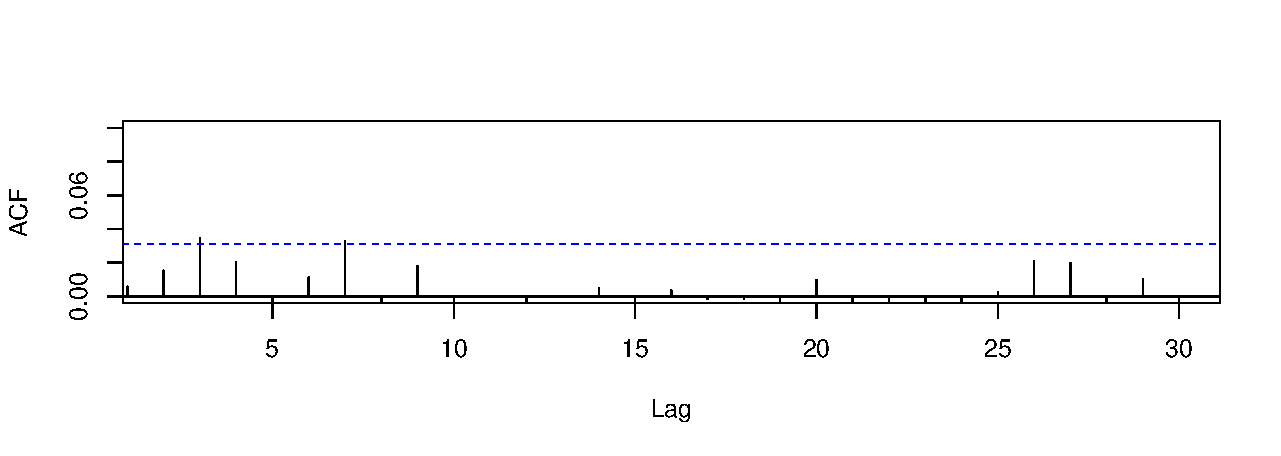
\includegraphics[width=1\linewidth]{theta_1_acf.pdf}
\end{figure}
\vspace{-0.5cm}


\subquestionwithpoints{3} Do we need to thin a certain number of initial samples? If yes, write the approximate iteration number. If no, write zero.

\iftoggle{solutions}{\inred{
8
}}{~\spc{0}}

Regardless of what you wrote for answers in (h) and (i), assume we do the necessary burning and thinning.

Below are the samples of $\theta_1$ given $\x$.  

\begin{figure}[h]
    \centering
    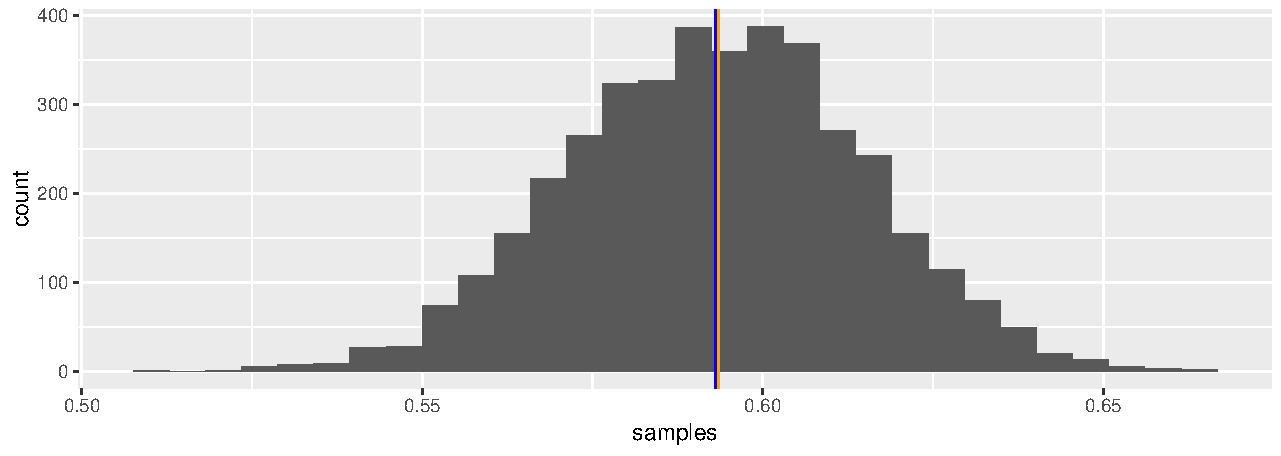
\includegraphics[width=0.9\linewidth]{theta_1s.pdf}
\end{figure}

\subquestionwithpoints{3}  Provide a CR$_{\theta_1, 95\%}$.

\iftoggle{solutions}{\inred{
$[.550,.635]$
}}{~\spc{0}}

\subquestionwithpoints{4} Decision $H_0: \theta_1 \leq 0.5$ at $\alpha = 5\%$ and provide justification.

\iftoggle{solutions}{\inred{
Reject $H_0$ because the Bayesian p-value is $\cprob{H_0}{\x} = \cprob{\theta_1 \leq 0.5}{\x} \approx 0 < \alpha$.
}}{~\spc{3}}
\pagebreak

Below are the samples of $\theta_2$ given $\x$.  

\begin{figure}[h]
    \centering
    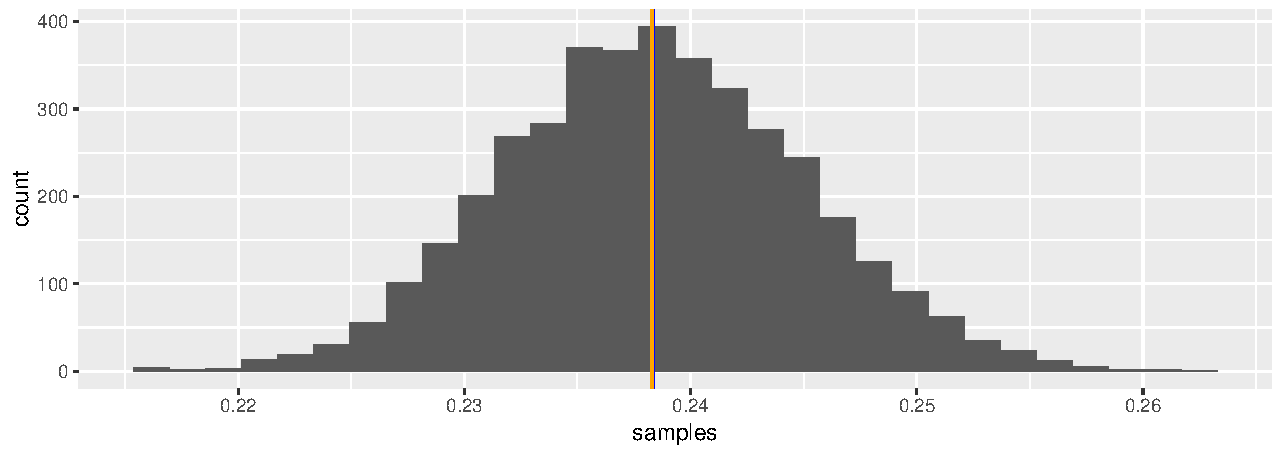
\includegraphics[width=0.9\linewidth]{theta_2s.pdf}
\end{figure}

\subquestionwithpoints{5} Decision $H_0: \theta_2 = 0.5$ at $\alpha = 5\%$ and provide justification.

\iftoggle{solutions}{\inred{
Reject $H_0$ because the Bayesian p-value is $\cprob{H_0}{\x} = \cprob{\theta_1 \in [0.5 \pm \delta]}{\x} \approx 0 < \alpha$ for any reasonable $\delta$.
}}{~\spc{2}}


\subquestionwithpoints{5} Estimate $\expe{X}$ to the nearest two decimals.

\iftoggle{solutions}{\inred{
\beqn
\expe{X} &=& \cexpe{X}{X = 0} \prob{X = 0} + \cexpe{X}{X > 0} \prob{X > 0} \\
&\approx& (0) \thetahathatmmse_1 + \parens{\frac{m\thetahathatmmse_2}{1 - (1-\thetahathatmmse_2)^{15}}} (1 - \thetahathatmmse_1) \\
&=& \parens{\frac{15 \cdot .238}{1 - (1-.238)^{15}}} (1 - .59) = 1.49
\eeqn
}}{~\spc{4}}

\subquestionwithpoints{5} Extra credit: Explain what you would do to test $H_0: \theta_1 \leq \theta_2$ at level $\alpha = 5\%$.

\iftoggle{solutions}{\inred{
Given the sampling chain where the first column is the samples of $\theta_1$ and the second column is $\theta_2$, I would create a third column with values equal to $\theta_1 - \theta_2$. I would then create a histogram of that column and estimate the proportion of samples less than zero. If the proportion is less than 5\%, I would reject $H_0$ (otherwise retain $H_0$).
}}{~\spc{6}}


\end{enumerate}


\pagebreak

\problem Consider the following observations where the + sign indicates censoring. The unit of measurements here is seconds.

\begin{verbatim}
0.012 0.030+ 0.039+ 0.064 0.073+ 0.153 0.203+ 0.349 0.493+ 0.844
\end{verbatim}

\begin{enumerate}

\subquestionwithpoints{5} First, ignore censoring. Create a table with the values of the $t_i$'s, $d_i$'s and $n_i$'s. Label the $n_i$ values as $n_0$, $n_1$, $n_2$, etc. If the value of the entry is zero or not applicable, you can leave the cell in the table blank. The first row is filled in for you.

\iftoggle{solutions}{
\begin{table}[h]
    \centering
    \inred{
\begin{tabular}{c|c|l}
    $t_i$ & $d_i$ & $n_i$ \\ \hline
    0     & 0          & $n_1 = 10$ \\
    0.012 & 1          & $n_2 = n_1 - 1 = 9$ \\
    0.030 & 1          & $n_3 = n_2 - 1 = 8$ \\
    0.030 & 1          & $n_4 = n_3 - 1 = 7$ \\
    0.064 & 1          & $n_5 = n_4 - 1 = 6$ \\
    0.073 & 1          & $n_6 = n_5 - 1 = 5$ \\
    0.153 & 1          & $n_7 = n_6 - 1 = 4$ \\
    0.203 & 1          & $n_8 = n_7 - 1 = 3$ \\
    0.349 & 1          & $n_9 = n_8 - 1 = 2$ \\
    0.493 & 1          & $n_{10} = n_9 - 1 = 1$ \\
    0.844 & 1          & $n_{11} = n_{10} - 1 = 0$ \\
\end{tabular}}
\end{table}
}{
\begin{table}[h]
    \centering
    \begin{tabular}{c|c|l}
$t_i$ &$d_i$ &$n_i$  \\\hline
    0     &  0  & $n_1$ = 10      \\
~~~~~~~~~  & ~~~ &  ~~~~~~~~~~~~~~~~~~~~~~~~~~~~~~~~~~~~~~~~~~~~~~~~~~~~~~~~~~~~  \\
&       & \\
&       & \\
&       & \\
&       & \\
&       & \\
&       & \\
&       & \\
&       & \\
&       & \\
&       & \\
&       & \\
&       & \\
&       & \\
&       & \\
&       & \\
&       & \\
&       & \\
&       & \\
    \end{tabular}
\end{table}
}


\subquestionwithpoints{5} Create a 95\% CI for survival past 0.5 seconds rounded to the nearest millisecond.

\iftoggle{solutions}{\inred{
\beqn
CI_{S(0.5), 95\%} &=& \bracks{~\doublehat{S}(0.5) \pm 1.96 \sqrt{\overn{\doublehat{S}(0.5) (1 - \doublehat{S}(0.5))}}~} \\
&=& \bracks{~0.1 \pm 1.96 \sqrt{\frac{0.1 (1 - 0.9)}{10}}~} \\
&=& \bracks{-0.086, 0.286} 
\eeqn
}}{~\spc{4}}
\pagebreak

\subquestionwithpoints{5} [i] What is wrong with the interval from (b)? [ii] Why did this happen? [iii] Could you use the bootstrap to fix this problem? [iv] What new problems would the bootstrap introduce?

\iftoggle{solutions}{\inred{
\begin{enumerate}[i]
    \item The lower bound is below zero. Survival times must be non-negative.
    \item Low sample size. $n = 10$ which is too small for the CLT to kick in.
    \item Yes
    \item The bootstrap is also approximate relying on large sample asymptotics. We have low sample size. So the bootstrap interval won't have accurate coverage.
\end{enumerate}
}}{~\spc{5}}

\subquestionwithpoints{5} Create a table with the values of the $t_i$'s, $s_i$'s, $d_i$'s,  $q_i$'s and $n_i$'s. Label the $n_i$ values as $n_0$, $n_1$, $n_2$, etc. If the value of the entry is zero or not applicable, you can leave the cell in the table blank. The first row is filled in for you.


\iftoggle{solutions}{
\begin{table}[h]
    \centering
    \inred{
    \begin{tabular}{c|c|c|c|l}
    $t_i$ & $s_i$ & $d_i$ & $q_i$ & $n_i$ \\ \hline
    0     &       & 0     &       & $n_1 = 10$ \\
    0.012 &       & 1     &       & $n_2 = n_1 - 1 - 1 - 1 = 7$ \\
          & 0.030 &       & 1     & \\
          & 0.039 &       & 1     & \\
    0.064 &       & 1     &       & $n_3 = n_2 - 1 - 1 = 5$ \\
          & 0.073 &       & 1     & \\
    0.153 &       & 1     &       & $n_4 = n_3 - 1 - 1 = 3$ \\
          & 0.203 &       & 1     & \\
    0.349 &       & 1     &       & $n_5 = n_4 - 1 - 1 = 1$ \\
          & 0.493 &       & 1     & \\
    0.844 &       & 1     &       & $n_6 = n_5 - 1 = 0$ \\
\end{tabular}}
\end{table}
}{
\begin{table}[h]
    \centering
    \begin{tabular}{c|c|c|c|l}
$t_i$&$s_i$&$d_i$&$q_i$&$n_i$  \\\hline
    0     &       &       &        & $n_1$ = 10      \\
~~~~~~~~~      & ~~~~~~~~~      & ~~~   & ~~~ & ~~~~~~~~~~~~~~~~~~~~~~~~~~~~~~~~~~~~~~~~~~~~~~~~~~~~~~~~~~~~  \\
&       &       &   &    \\
&       &       &   &    \\
&       &       &   &    \\
&       &       &   &    \\
&       &       &   &    \\
&       &       &   &    \\
&       &       &   &    \\
&       &       &   &    \\
&       &       &   &    \\
&       &       &   &    \\
&       &       &   &    \\
&       &       &   &    \\
&       &       &   &    \\
&       &       &   &    \\
&       &       &   &    \\
&       &       &   &    \\
&       &       &   &    \\
&       &       &   &    \\
&       &       &   &    \\
    \end{tabular}
\end{table}
}
\pagebreak


\subquestionwithpoints{8} Graph the Kaplan-Meier survival curve estimate on the gridlines below. Mark censored observations with a vertical dash on the survival curve estimate. Use open dots and closed dots where appropriate. \textit{Label the axes appropriately}. If you do not know who to do this, draw as much as you know how to do so you can answer the following questions in this problem.

\iftoggle{solutions}{
\inred{
To generate the Kaplan-Meier survival curve estimate, we need to compute the step function's points of discontinuity which are the values of the product limit estimator for all $t_i$:
\beqn
\footnotesize
\doublehat{S}(t_1) = \doublehat{S}(0.012) &=& p_1 = 1 - \frac{d_1}{n_1} = 1 - \oneover{10} = 0.9 \\
%%%%%%
\doublehat{S}(t_2) = \doublehat{S}(0.064) &=& p_1 p_2 = p_1 \parens{1 - \frac{d_2}{n_2}} = 0.9 \parens{1 - \oneover{7}} = 0.9 \cdot 0.857 = 0.771\\
%%%%%%
\doublehat{S}(t_3) = \doublehat{S}(0.153) &=& p_1 p_2 p_3 = p_1 p_2 \parens{1 - \frac{d_3}{n_3}} = 0.771 \parens{1 - \oneover{5}} = 0.771 \cdot 0.8 = 0.617\\
%%%%%%
\doublehat{S}(t_4) = \doublehat{S}(0.349) &=& p_1 p_2 p_3 p_4 = p_1 p_2 p_3 \parens{1 - \frac{d_4}{n_4}} = 0.617 \parens{1 - \oneover{3}} = 0.617 \cdot 0.667 = 0.411\\
%%%%%%
\doublehat{S}(t_5) = \doublehat{S}(0.844) &=& p_1 p_2 p_3 p_4 p_5 = p_1 p_2 p_3 p_4 \parens{1 - \frac{d_5}{n_5}} = 0.411 \parens{1 - \oneover{1}} = 0.411 \cdot 0 = 0\\
\eeqn
}
\vspace{-1.2cm}
\begin{figure}[h]
    \centering
    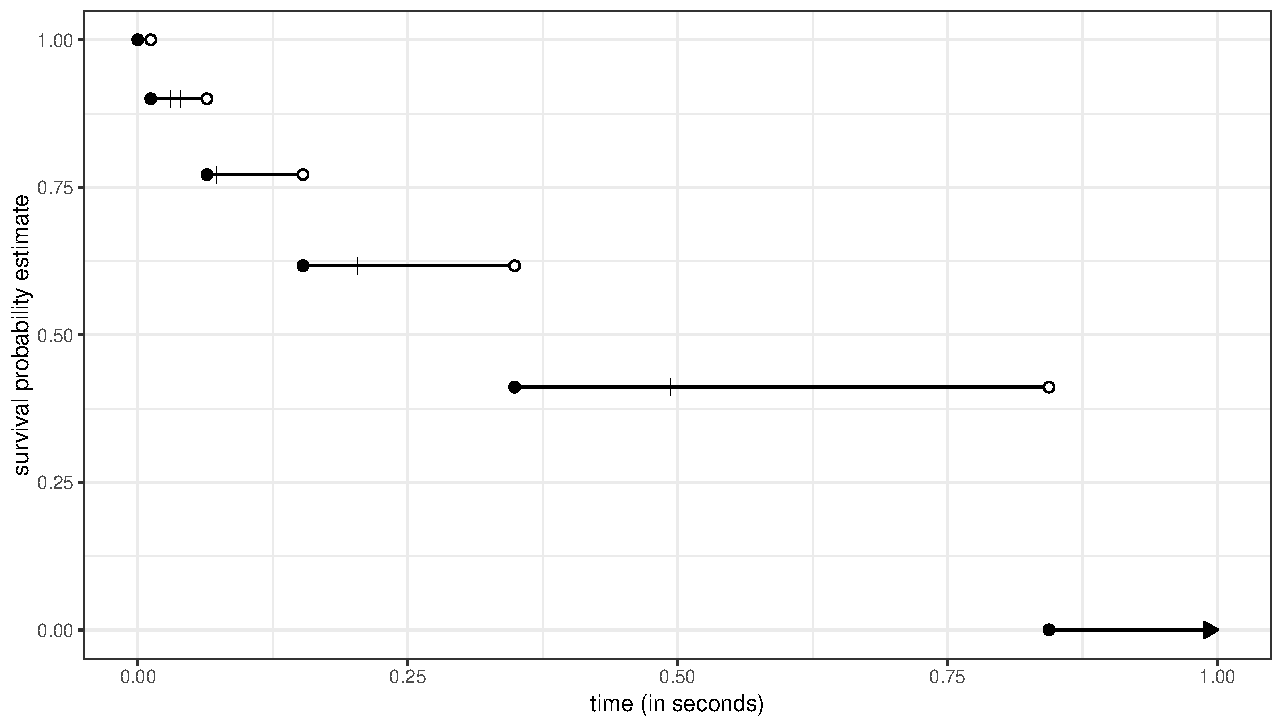
\includegraphics[width=1.1\linewidth]{KM.pdf}
\end{figure}


}{
\begin{figure}[h]
    \centering
    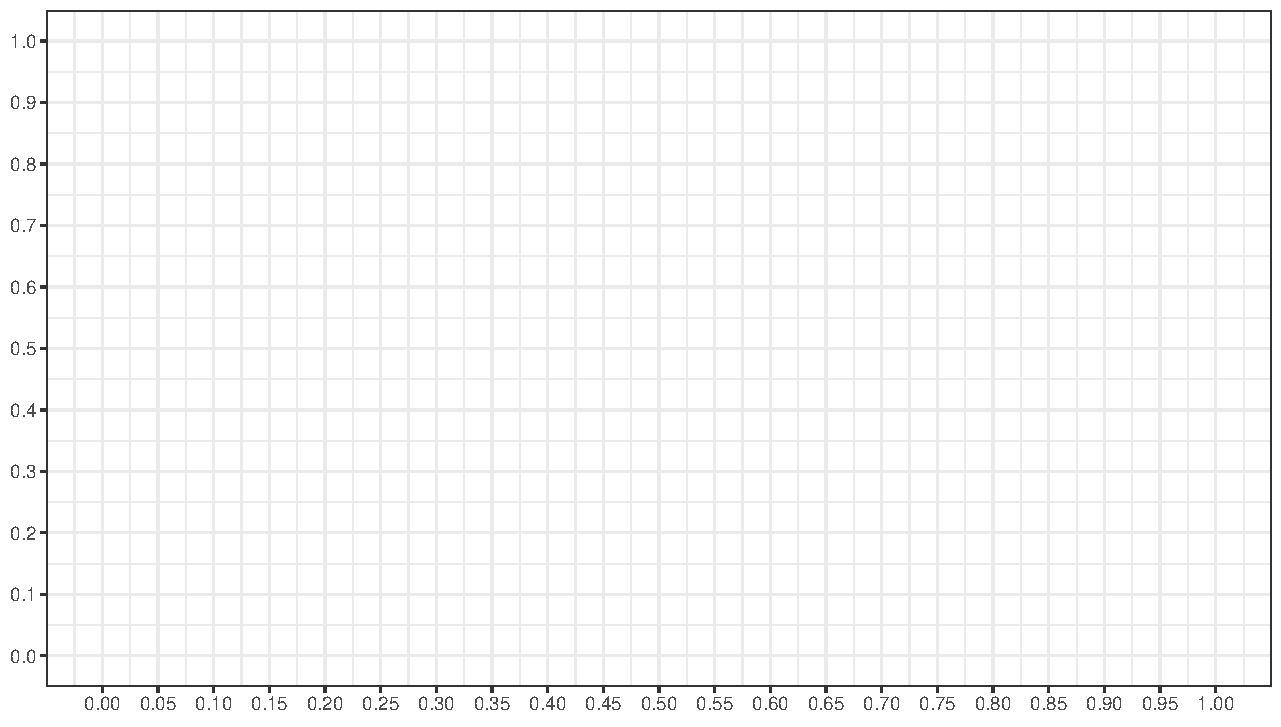
\includegraphics[width=1.1\linewidth]{blank_survival.pdf}
\end{figure}
~\spc{6}
}

\subquestionwithpoints{2} Using the plot from (e), estimate the median survival. If you didn't put an answer in (e), make up a legal survival curve and answer based on that.

\iftoggle{solutions}{\inred{
0.349, the $y$ corresponding to the minimum time $\doublehat{S}(y) < 0.5$.
}}{~\spc{1}}
\pagebreak

\end{enumerate}

\problem We are interested in the differential survival (measured in days) of two groups of lung cancer patients differentiated by a cutoff of their beginning Karnovsky performance score rated by a physician. Group 1 is defined as those above the cutoff which have \qu{good performance} and group 0 is defined as those below the cutoff which have \qu{bad performance}. There are $n_1 = 123$ subjects with good performance and $n_0 = 44$ subjects with bad performance. Below are the KM survival curve estimates for both groups. The vertical dash signs indicate a censored observation. In the legend, \qu{x} means \qu{group}. Let $Y_0$ denote the SDGP for group 0 and let $Y_1$ denote the SDGP for group 1.

\vspace{-0.4cm}
\begin{figure}[h]
    \centering
    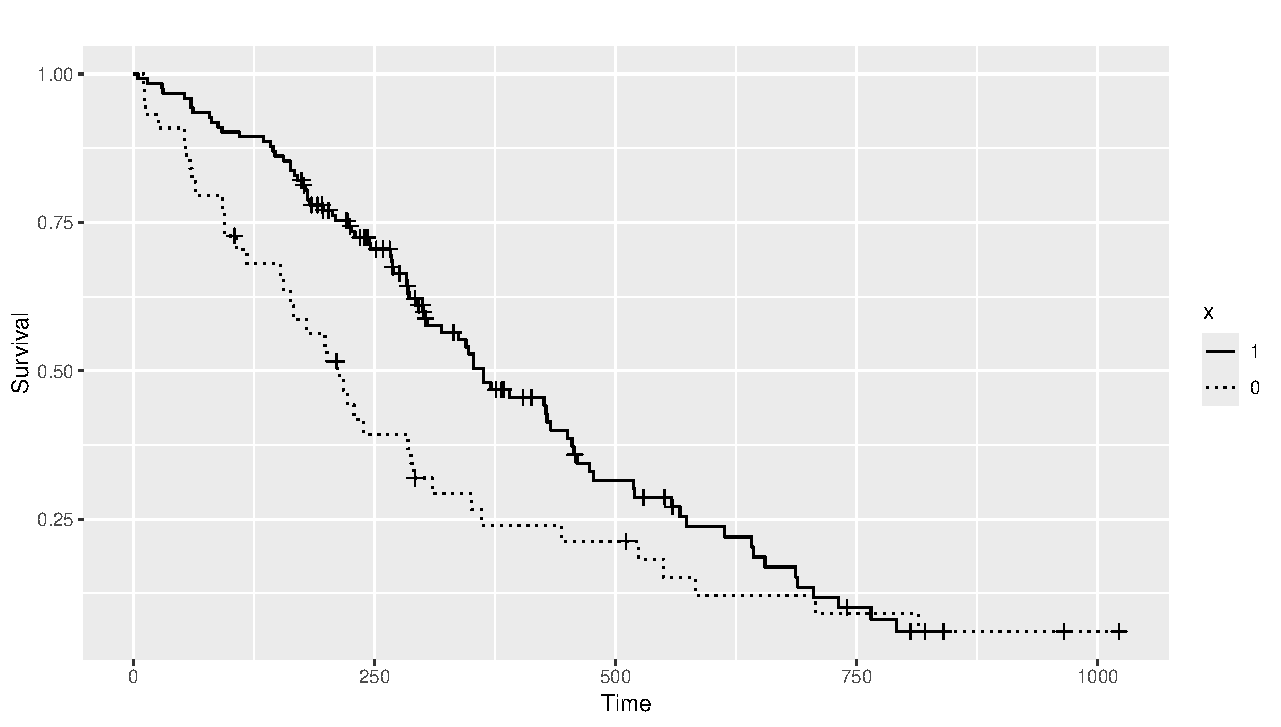
\includegraphics[width=0.9\linewidth]{kms.pdf}
    \label{fig:enter-label}
\end{figure}
\FloatBarrier
\vspace{-0.8cm}

\begin{enumerate}[(a)]
\subquestionwithpoints{2} Estimate $S_{Y_1}(500d) - S_{Y_0}(500d)$

\iftoggle{solutions}{\inred{
10\%
}}{~\spc{-0.7}}

\subquestionwithpoints{2} Using just a visual inspection of the KM survival curve estimates, make a decision about $H_0: \text{Med}[Y_0] = \text{Med}[Y_1]$. Justify your answer.

\iftoggle{solutions}{\inred{
Reject $H_0$ because the median survival in group 1 looks significantly larger than the median survival in group 0.
}}{~\spc{1}}

Below is the output from the function \texttt{survdiff}:

\begin{verbatim}
          N Observed Expected (O-E)^2/E (O-E)^2/V
x=0  44       38     27.2      4.29      5.65
x=1 123       82     92.8      1.26      5.65
\end{verbatim}

\subquestionwithpoints{3} Make a principled decision about $H_0: f_{Y_0}(y) = f_{Y_1}(y)$. Justify your answer fully.

\iftoggle{solutions}{\inred{
Using the log rank test at $\alpha = 5\%$, $\doublehat{\phi} = 4.29 + 1.26 = 5.7 > 1.96^2 = 3.84 \Rightarrow$ reject $H_0$.
}}{~\spc{0}}

\end{enumerate}
\pagebreak


\problem Fisher introduced the permutation test (often called the randomization test) in his 1935 book, The Design of Experiments. The dataset he famously used was Charles Darwin’s data on the heights of Zea mays (corn) plants. Darwin had grown 15 pairs of corn plants: one cross-fertilized and one self-fertilized. He grew them in the same pots to control for environmental differences. Below is the original data Fisher used: %Fisher used this paired data to demonstrate that you could evaluate the null hypothesis by calculating the test statistic across all $2^{15}$ (or 32,768) possible permutations of the signs of the differences. 

\begin{table}[ht]
\centering
\begin{tabular}{crr}
\hline
$i$ & Group 1: Cross-fertilized (inches) & Group 2: Self-fertilized (inches) \\
\hline
1 & 23.500 & 17.375 \\
2 & 12.000 & 20.375 \\
3 & 21.000 & 20.000 \\
4 & 22.000 & 20.000 \\
5 & 19.125 & 18.375 \\
6 & 21.500 & 18.625 \\
7 & 22.125 & 18.625 \\
8 & 20.375 & 15.250 \\
9 & 18.250 & 16.500 \\
10 & 21.625 & 18.000 \\
11 & 23.250 & 16.250 \\
12 & 21.000 & 18.000 \\
13 & 22.125 & 12.750 \\
14 & 23.000 & 15.500 \\
15 & 12.000 & 18.000 \\
\hline
Average &20.192 & 17.575 \\
\end{tabular}
\end{table}

\noindent We will ignore the pairing of the data (since we didn't discuss this in class) so we will not be duplicating Fisher's original statistical test. We will be doing a permutation test and assuming a test statistic of $\xbar_1 - \xbar_2$.

\begin{enumerate}[(a)]
\subquestionwithpoints{2} How many permutations exist in this scenario?

\iftoggle{solutions}{\inred{
$\displaystyle\binom{30}{15}$
}}{~\spc{0}}

\subquestionwithpoints{3} What would be a potential weakness of using the test statistic $\xbar_1 - \xbar_2$?

\iftoggle{solutions}{\inred{
If the DGP's for group 1 and group 2 have equal expectations but different variances, this test would have very little power.
}}{~\spc{2}}

\pagebreak

\noindent Below is a histogram of 100,000 test statistics each computed on different permutations of the data.

\begin{figure}[h]
    \centering
    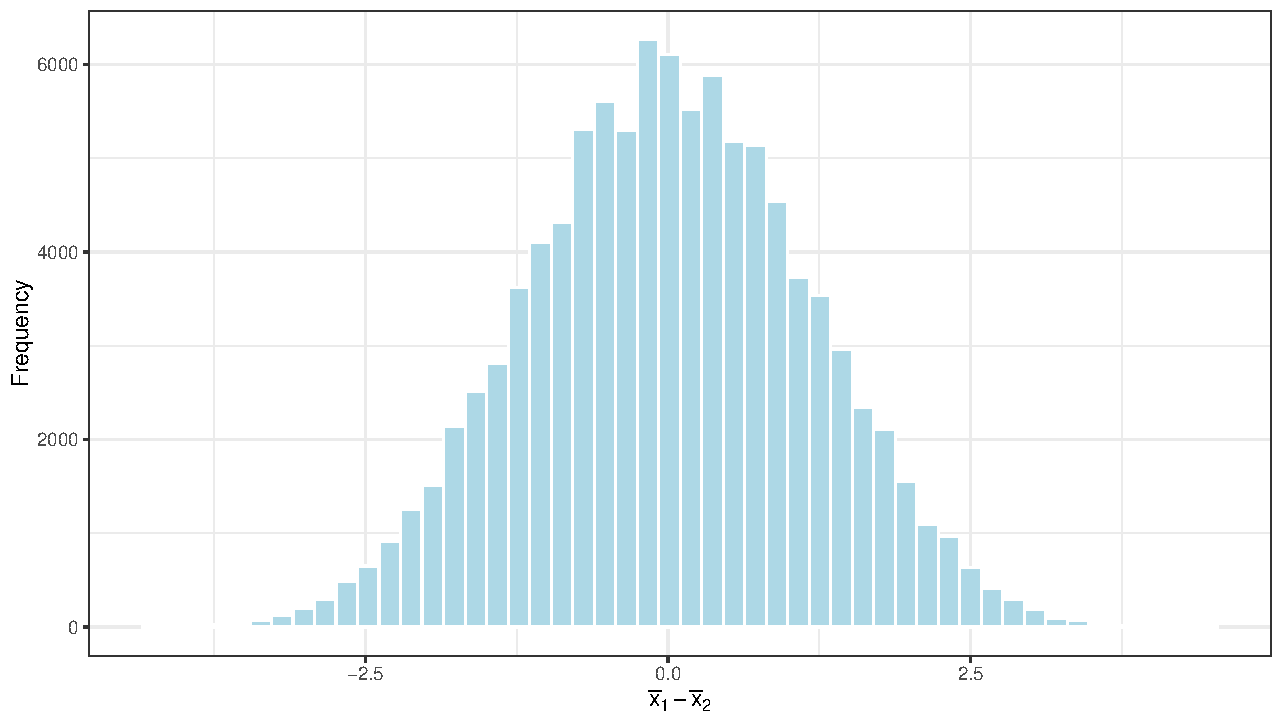
\includegraphics[width=1\linewidth]{perm.pdf}
\end{figure}


\subquestionwithpoints{3} At $\alpha = 5\%$, test $H_0: \text{DGP}_1 = \text{DGP}_2$. Justify your answer fully.

\iftoggle{solutions}{\inred{
The 95\% retainment region seems to be at $[-2.5,2.5]$ and the observed statistic is 20.192 - 17.575 = 2.617 hence we reject $H_0$.
}}{~\spc{3}}

\subquestionwithpoints{3} Estimate Fisher's p-value for the test in (c). Your answer must comport with (c) for full credit.

\iftoggle{solutions}{\inred{
Since 2.617 is just barely greater than the edge of the retainment region, integrating the area above would be slightly less than 2.5\% maybe $\approx$ 2\%. Multiplying by two for the two sided test would give us an estimate of $4\%$.
}}{~\spc{3}}


\end{enumerate}
\end{document}



\problem Consider the following rv and some of its properties:

\beqn
X \sim \text{Gamma}(\theta_1, \theta_2) := \frac{\theta_2^{\theta_1}}{\Gammaf{\theta_1}} x^{\theta_1 - 1} e^{-\theta_2 x}\indic{x > 0},~~~\theta_1 > 0,~~ \theta_2 > 0,~~ \expe{X} = \frac{\theta_1}{\theta_2}, ~~ \var{X} = \frac{\theta_1}{\theta_2^2}
\eeqn

\noindent We realize $n = 100$ iid realizations from this DGP and calculate the following quantities rounded to two decimals:

\beqn
\xbar := \oneover{n} \sum_{i=1}^n x_i &=& 3.51 \\%, ~~~~~~ \oneover{n} \sum_{i=1}^n x_i^6 = 3071.00  \\
\oneover{n} \sum_{i=1}^n x_i^2 &=& 7.89 \\%, ~~~~~~ \oneover{n} \sum_{i=1}^n x_i^7 = 16475.31 \\
\oneover{n} \sum_{i=1}^n x_i^3 &=& 29.62 \\%, ~~~~~~ \oneover{n} \sum_{i=1}^n x_i^8 = 91664.09  \\
\oneover{n} \sum_{i=1}^n x_i^4 &=& 127.21 \\ %, ~~~~~~ \oneover{n} \sum_{i=1}^n x_i^9 = 523306.42  \\
\oneover{n} \sum_{i=1}^n x_i^5 &=& 602.66 \\%, ~~~~~~ \oneover{n} \sum_{i=1}^n x_i^{10} = 3042898.00  \\
\eeqn

\begin{enumerate}[(a)]

\subquestionwithpoints{3} Observing $n = 100$ iid realizations from this DGP is equivalent to sampling an SRS of $n = 100$ from a population with which propert(ies)?

\iftoggle{solutions}{\inred{
Infinitely large
}}{~\spc{1}}

\subquestionwithpoints{3} Find the method of moments (MM) estimator for $\expe{X}$.

\iftoggle{solutions}{\inred{
$\Xbar$
}}{~\spc{1}}

\subquestionwithpoints{3} What is the MM estimate for $\expe{X}$? Round to the nearest two decimals.

\iftoggle{solutions}{\inred{
$\xbar = 2.72$
}}{~\spc{1}}

\pagebreak

\subquestionwithpoints{6} Find the MM estimator for $\theta_2$.

\iftoggle{solutions}{\inred{
\beqn
&& \expe{X} = \muhat_1 = \frac{\theta_1}{\theta_2}, ~~\var{X} = \muhat_2 - \muhat_1^2 = \frac{\theta_1}{\theta_2^2} \\
&& \mathimplies \theta_1 = \muhat_1 \theta_2 \mathimplies \muhat_2 - \muhat_1^2 = \frac{\muhat_1 \theta_2}{\theta_2^2} = \frac{\muhat_1}{\theta_2} \mathimplies \thetahatmm_2 = \frac{\muhat_1}{\muhat_2 - \muhat_1^2}
%\muhat_2 - \squared{\frac{\theta_1}{\theta_2}} = \frac{\theta_1}{\theta_2^2} \\
\eeqn
}}{~\spc{7}}

\subquestionwithpoints{3} What is the MM estimate for $\theta_2$? Round to the nearest two decimals.

\iftoggle{solutions}{\inred{
\beqn
\thetahathatmm_2 = \frac{\muhathat_1}{\muhathat_2 - \muhathat_1^2} = \frac{3.51}{7.89 - 3.51^2} = -0.79
\eeqn
}}{~\spc{1}}

\subquestionwithpoints{4} Does the MM estimate for $\theta_2$ make sense? Why or why not?

\iftoggle{solutions}{\inred{
No, it is negative and the parameter space for $\theta_2$ is positive.
}}{~\spc{1}}


\subquestionwithpoints{5} Find a MM estimator for $\theta_1$.

\iftoggle{solutions}{\inred{

We use intermediate results and our result found in (d)

\beqn
&& \theta_1 = \muhat_1 \theta_2, ~~~\thetahatmm_2 = \frac{\muhat_1}{\muhat_2 - \muhat_1^2} \mathimplies \thetahatmm_1 = \muhat_1 \parens{\frac{\muhat_1}{\muhat_2 - \muhat_1^2}} = \frac{\muhat_1^2}{\muhat_2 - \muhat_1^2}
\eeqn
}}{~\spc{6}}
\pagebreak

Now consider the scenario where we know that the value of $\theta_1 = 4$. The constant in the denominator can be calculated to be 6. Now, there is only one parameter, so we simplify the expression and just denote it $\theta$. Thus,

\beqn
X \sim \text{Gamma}(4, \theta) := \frac{\theta^{4}}{6} x^3 e^{-\theta x}\indic{x > 0}
\eeqn

\subquestionwithpoints{7} Show that $\thetahatmle = \frac{4}{\Xbar}$ for general sample of size $n$. All data is properly realized and are positive values and thus you can drop the indicator term during your calculation.

\iftoggle{solutions}{\inred{

\beqn
\mathcal{L}(\theta; \X) &=& \prod_{i=1}^n \frac{\theta^{4}}{6} X_i^3 e^{-\theta X_i} = \frac{\theta^{4n}}{6^n} X_i^{3n} e^{-\theta \displaystyle\sum_{i=1}^n X_i} \\
\ell(\theta; \X) &=& 4n \natlog{\theta} - n \natlog{6} - \theta \displaystyle\sum_{i=1}^n X_i \\
\ell'(\theta; \X) &=& \frac{4n}{\theta} - \sum_{i=1}^n X_i ~~{\buildrel \text{set} \over =}~~ 0 \mathimplies \frac{4n}{\theta} = \sum_{i=1}^n X_i \mathimplies \thetahatmle = \frac{4n}{\sum_{i=1}^n X_i} = \frac{4}{\Xbar}
\eeqn
}}{~\spc{8}}

\subquestionwithpoints{3} Show that this MLE is indeed a maximum of the log-likelihood by using a second derivative check. Explain your reasoning.

\iftoggle{solutions}{\inred{

\beqn
\ell''(\theta; \X) = -\frac{4n}{\theta^2} < 0 ~~~\text{since $n \in \naturals$, the sample size and $\theta > 0$, the parameter space}
\eeqn
}}{~\spc{6}}

\pagebreak

\subquestionwithpoints{6} Derive the CRLB for $\theta$ in the DGP $X \sim \text{Gamma}(4, \theta)$.

\iftoggle{solutions}{\inred{

\beqn
\ell''(\theta; \X) = -\frac{4n}{\theta^2},~~ I_n(\theta) = \expe{-\ell''(\theta; \x)} = \expe{-\parens{-\frac{4n}{\theta^2}}} = \frac{4n}{\theta^2},~~~ \var{\thetahat} \geq \frac{1}{I_n(\theta)} = \frac{\theta^2}{4n}
\eeqn
}}{~\spc{12}}


\subquestionwithpoints{1} It can be shown that 

\beqn
\expe{\thetahatmle} = \frac{4n}{4n-1} \theta.
\eeqn

Is $\thetahatmle$ unbiased? Yes or no.

\iftoggle{solutions}{\inred{
No
}}{~\spc{0}}
\pagebreak

\subquestionwithpoints{6} It can be shown that 

\beqn
\var{\thetahatmle} = \frac{(4n)^2}{(4n-1)^2(4n-2)} \theta^2.
\eeqn

Calculate $\mse{\thetahatmle}$ as a function of $n$ and $\theta$. Simplify as much as you can.


\iftoggle{solutions}{\inred{
\beqn
\mse{\thetahatmle} &=& \bias{\thetahatmle}^2 + \var{\thetahatmle} \\
&=& \parens{\frac{4n}{4n-1} \theta - \theta}^2 + \frac{(4n)^2}{(4n-1)^2(4n-2)} \theta^2 \\
&=& \parens{\parens{\frac{4n}{4n-1}  - 1}^2 + \frac{(4n)^2}{(4n-1)^2(4n-2)}} \theta^2 \\
&=& \parens{\parens{\frac{1}{4n-1}}^2 + \frac{(4n)^2}{(4n-1)^2(4n-2)}} \theta^2 \\
&=& \parens{\frac{(4n-2)}{(4n-1)^2 (4n-2)} + \frac{(4n)^2}{(4n-1)^2(4n-2)}} \theta^2 \\
&=& \frac{(4n)^2 + 4n-2}{(4n-1)^2(4n-2)} \theta^2 \\
\eeqn
}}{~\spc{11}}

\subquestionwithpoints{5} Under squared error loss, compute $\displaystyle\sup_{\theta \in \Theta} \braces{R(\thetahatmle, \theta)}$.

\iftoggle{solutions}{\inred{
$\infty$
}}{~\spc{2}}

\end{enumerate}
\pagebreak

\problem Consider a survey of iPhoneness. $n=27$ students were chosen outside of Kiely Hall on Tuesday afternoon, Sept 30, 2025 were asked if they had an iPhone ($x_i = 1$) or not ($x_i = 0$). In total, 23 students had iPhones. We wish to infer about the population of all QC undergraduate students.


\begin{enumerate}

\subquestionwithpoints{4} Is this sample an SRS from the population of interest? Why or why not?

\iftoggle{solutions}{\inred{
You can say yes but you must argue that students at CUNY take classes at uniformly random times in uniformly random locations. Likely the answer is no because if you are on campus on Tuesday afternoon you are not a weekend student (those of which may be different socioeconomically). Also, Kiely Hall has more STEM classes than other buildings so those students may not be representative of all undergraduates either.
}}{~\spc{5}}

Regardless of what you wrote in (a), consider this sample to be an SRS from the population of interest for the rest of this question.


\subquestionwithpoints{9} The US mean countrywide proportion of iPhones is estimated to be 62\%. Prove via a hypothesis test at $\alpha = 5\%$ using the one-proportion Z-test that the QC population has higher iPhone proportion than the countrywide mean. Your answer must include a clear setup of the two hypotheses, a retainment region and a decision. Do not interpret the decision nor find Fisher's $p_{val}$. Those will be asked in subsequent questions.

\iftoggle{solutions}{\inred{
$H_0: \theta \leq .62,~H_a: \theta > .62$. We can then build the retainment region for $\alpha=0.05$ with the relevant $z_{1 - \alpha} = 1.65$ as it's one sided. So 

\beqn
RET = \Bigg(-\infty, \theta_0 + z_{1 - \alpha} \sqrt{\overn{\theta_0 (1 - \theta_0)}}\Bigg] = \Bigg(-\infty, .62 + 1.65 \sqrt{\frac{.62 (1-0.62)}{27}}\Bigg] = (-\infty, .774] 
\eeqn

Now we calculate $\xbar = 23/27 = .852 \notin RET$ hence $H_0$ is rejected.
}}{~\spc{6}}
\pagebreak

\subquestionwithpoints{4} Interpret your decision from the previous question.

\iftoggle{solutions}{\inred{
There is statistically significant evidence to conclude that the QC population has a higher iPhone proportion than the countrywide mean.
}}{~\spc{3}}


\subquestionwithpoints{2} If your decision was an error, what type of error was it?

\iftoggle{solutions}{\inred{
Type I
}}{~\spc{0}}

\subquestionwithpoints{6} Represent Fisher's $p_{val}$ by using the $\Phi$ notation (i.e. the CDF of the standard normal).

\iftoggle{solutions}{\inred{
\beqn
p_{val} &=& \cprob{\thetahat > \thetahathat}{H_0} \\
&=& \cprob{\thetahat > .852}{\thetahat \sim \normnot{.62}{\frac{.62 (1-0.62)}{27}}} \\
&=& \prob{\frac{\thetahat - .62}{\sqrt{\frac{.62 (1-0.62)}{27}}} > \frac{.852 - .62}{\sqrt{\frac{.62 (1-0.62)}{27}}}} \\
&=& \prob{Z > 2.48} \\
&=& 1 - \Phi(2.48)
\eeqn
}}{~\spc{8}}


\subquestionwithpoints{3} Why is the $p_{val}$ from the previous question approximate?

\iftoggle{solutions}{\inred{
We used the standard normal as the result of the CLT which is approximate for any finite sample size.
}}{~\spc{3}}
\pagebreak

\subquestionwithpoints{1} If you wanted an exact test, what is the name of the test would you use?

\iftoggle{solutions}{\inred{
Binomial Exact Test
}}{~\spc{0}}


\subquestionwithpoints{3} In order to calculate the power of this test, what information would you need?

\iftoggle{solutions}{\inred{
The true distribution of $\thetahat$.
}}{~\spc{1}}


\subquestionwithpoints{3} If you ran the test with $\alpha = 6\%$ instead of the original 5\%, would power increase or decrease?

\iftoggle{solutions}{\inred{
increase
}}{~\spc{0}}

\subquestionwithpoints{5} If the null hypothesis were true, as the sample size approaches infinity, what would the decision of the test be?

\iftoggle{solutions}{\inred{
You would still fail to reject. You are only guaranteed to reject if the null is false (even by a hairbreadth $\delta$).
}}{~\spc{3}}

\subquestionwithpoints{5} In order to calculate a 95\% CI for $\theta$, what specific information do you need? Note: this is a difficult question.

\iftoggle{solutions}{\inred{
When inverting the test, you'll see that you need the actual value of $\theta$ as the standard error of $\thetahat$ is $\sqrt{\theta(1-\theta) / n}$. (This is impossible as $\theta$ is unknown and hence why we did not yet cover the CI for the proportion).
}}{~\spc{3}}



\end{enumerate}


\end{document}
